\documentclass[final,dvipsnames]{beamer}
%% Possible paper sizes: a0, a0b, a1, a2, a3, a4.
%% Possible orientations: portrait, landscape
%% Font sizes can be changed using the scale option.
\usepackage[size=a0,orientation=portrait,scale=1.5,debug]{beamerposter}
%\graphicspath{{./img/}}
%\mode<presentation>\usetheme{inriaposter}

%\makeatletter
\usetheme{LLT-poster}
\usecolortheme{ComingClean}
%\usecolortheme{Entrepreneur}
%\usecolortheme{ConspiciousCreep}  %% VERY garish.
\usepackage[utf8]{inputenc}
\usepackage[T1]{fontenc}

%\usepackage{libertine}
\usepackage[scaled=1]{inconsolata}
%\usepackage[libertine]{newtxmath}
\usepackage{amsmath,amsfonts,amssymb,pxfonts,eulervm,xspace}
\usepackage{graphicx,subfigure,comment,tikz}
\usepackage{array}
\usepackage{adjustbox}
\usepackage{framed}
\usepackage{mdframed}
\usepackage{multirow}
\usepackage{xcolor}


\newcommand{\myemph}[1]{\textcolor{blue}{#1}}
\newcommand{\myemphh}[1]{\textbf{\textcolor{blue}{#1}}}



\newcommand{\mycolbackwhite}[1]{
\hspace*{.01\linewidth}\begin{minipage}{.96\linewidth}
\begin{mdframed}[backgroundcolor=white!10,linewidth=1pt]
\vspace{10pt}
#1
\vspace{10pt}
\end{mdframed}
\end{minipage}
}
\DeclareMathOperator\supp{supp}
\DeclareMathOperator\argmin{argmin}
\DeclareMathOperator\Bern{Bern}
\author[Martin.Gjorgjevski@gipsa-lab.grenoble-inp.fr]{Martin Gjorgjevski}
\title{The Graphical Nadaraya Watson Estimator on Latent Postion Models}
\institute{GIPSA-lab, Grenoble}


\usepackage[style=alphabetic-verb]{biblatex}
\addbibresource{references.bib}

\begin{document}
\begin{frame}
\begin{columns}[T]
%%%% First Column
\begin{column}{0.38\textwidth}

\begin{block}{Summary}
\begin{itemize}
\item We derive \textbf{sample complexities} and \textbf{generalization bounds} for a signal averaging estimator on graphs
\item  Analysis valid for general  \myemphh{Latent Position Models}
\end{itemize}
\end{block}
\begin{block}{Notation}
All random variables belong to a joint probability space $(\Omega,\mathcal{F},\mathbb{P})$
\vspace{20pt}
\begin{itemize}
    \item $\mathbb{E}(F(X,X_1,..,X_n,X,U_1,U_2,...,U_n,\epsilon_1,...,\epsilon_n)$- expectation taken over every variable 
    \item $\mathbb{E}_{x} (\cdot)=\mathbb{E}(\cdot|X=x)$ conditional expectation 
    \item $d_n(x)=\mathbb{E}_{x}(\sum_{i=1}^n a(X,X_i))$-local expected degree at $x\in\mathbb{R}^d$
    \item $b_n(f,x)=\begin{cases}
    \frac{\int f(z)k_n(x,z)p(z)dz}{\int k_n(x,z)p(z)dz} \quad &\text{if}\ d_n(x)> 0\\
    0 \quad &\text{otherwise}\\
    \end{cases}$
    \item $Q=\supp{p}$
\end{itemize}
\end{block}

\begin{block}{The GNW Estimator}
\begin{equation}
    \hat{f}_{GNW}(X)=\begin{cases}
    \frac{\sum_{i=1}^n Y_i a(X,X_i)}{\sum_{i=1}^n a(X,X_i)} \quad &\text{if}\,\sum a(X,X_i)\neq 0\\
    0 \quad &\text{otherwise}\\
    \end{cases}
\end{equation}
\vspace{20pt}
\begin{itemize}
    \item \textit{How does} $\mathbb{E}_{x}(\hat{f}_{GNW}(X)-b_n(f,X))^2$ \textit{depend on} $d_n(x)$?
    \item \textit{For \textbf{convolutional kernels} and \myemphh{smooth signals},   
    how does} $\mathbb{E}
(\hat{f}_{GNW}(X)-f(X))^2$ \textit{depend on the bandwith} $h_n$?
\end{itemize}

\begin{figure}
    \centering
   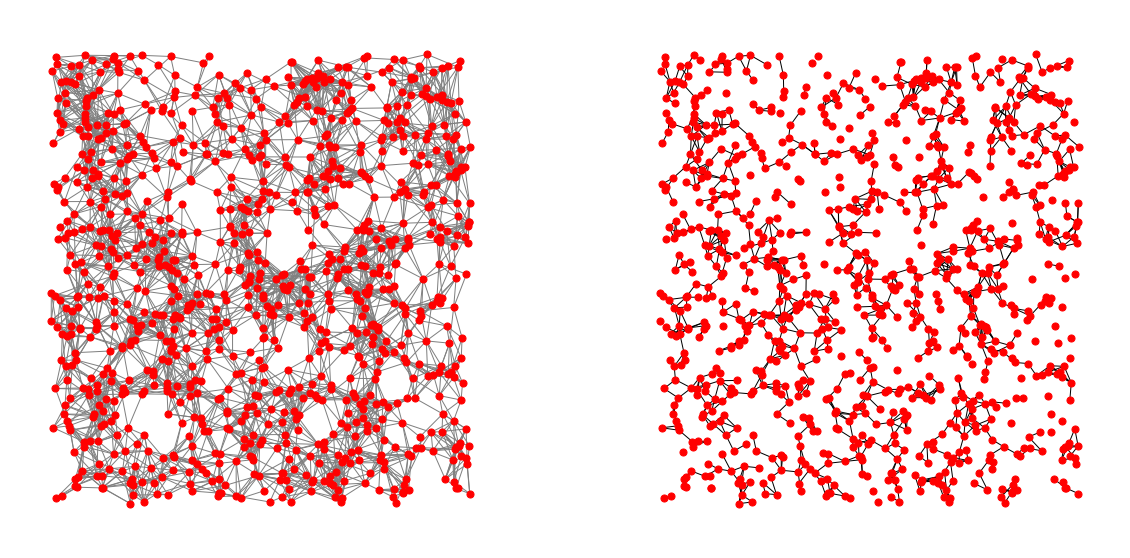
\includegraphics[width=1\textwidth]{fresh_for_marseille.png}

    \caption{Left- Graph with $\sim \log n$ average degree, Right- Graph with $\sim \log(\log(n))$ average degree}
    \label{fig:sparse_graphs}
\end{figure}
\end{block}

\begin{block}{MISE bound for convolutional kernels}
Convolutional kernels $k_n(x,z)=K(\frac{x-z}{h_n})$ with $K\colon\mathbb{R}^d\to [0,1]$, $h_n>0$.
\vspace{20pt}
Going from $\mathbb{E}_{x}(\cdot)$ to $\mathbb{E}(\cdot)$:
\vspace{20pt}
\begin{itemize}
    \item Bounds on $|b_n(f,x)-f(x)|$ (the \myemphh{bias} term) 
    \item Asymptotically $d_n(x)\sim nh_n^dp(x)$ (\textbf{Lebesgue Density theorem})
\end{itemize}
\vspace{20pt}
Nonasimptotically, the following holds:
\vspace{20pt}
\mycolbackwhite{
\vspace{20pt}
\begin{itemize}
    \item $K$ compactly supported 
    \item $p(x)\geq p_0>0$ on $Q$ and $Q$ \textit{satisfies \myemph{interior cone con dition}}
    \item f is $\alpha$ Hölder continnous on $Q$
        \end{itemize}

        then for sufficiently small bandwiths $h_n$
        \begin{equation*}
            \mathbb{E}(\hat{f}_{GNW}(X)-f(X))^2\leq C_1(\alpha)h_n^{\alpha}+\frac{C(B,\sigma)}{nh_n^d}
        \end{equation*}
        }
\end{block}
\end{column}

%%%% Second Column
\begin{column}{.6\textwidth}
\begin{block}{Framework}

\textit{Latent Position Models}:
\begin{figure}
    \centering
    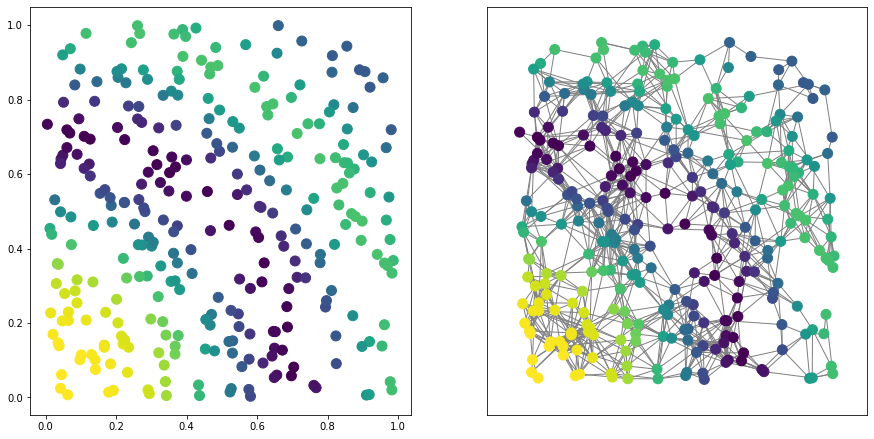
\includegraphics[width=\textwidth]{lpm_image_correct.png}
    \caption{Left- latent positions, Right - Latent Graph Random Graph}
    \label{fig:my_label}
\end{figure}
\begin{itemize}
    \item $X_1,...X_n,X$ i.i.d. $\sim p$, $p$ a density on $\mathbb{R}^d$
    \textit{\textbf{not observed}}
    \item $k_n:\mathbb{R}^d\to [0,1]$ probability kernel 
    \item $a(X_i,X_j)=bern(k_n(X_i,X_j))\colon=\mathbb{I}(k_n(X_i,X_j)\leq U_{i,j})$
    \item $Y_i-f(X_i)+\epsilon_i$, $\epsilon=(\epsilon_1,...,\epsilon_n)$ indepednent from $(X_1,...,X_n)$, $\mathbb{E}\epsilon_i=0$, $\mathbb{E}\epsilon_i^2
    =\sigma^2<\infty$
\end{itemize}

\end{block}



\begin{block}{Sharp Variance Bound}

\mycolbackwhite{Suppose that $f\colon\mathbb{R}^d\to\mathbb{R}$ is such that $||f||_{\infty}\leq B$ and $\mathbb{E}(\epsilon_1^2)=\sigma^2>0$. Then
\begin{equation*}
    \frac{\sigma^2(1-e^{-d_n(x)})}{d_n(x)}\leq \mathbb{E}(\hat{f}_{GNW}(x)-b_n(f,x))^2\leq \frac{C(B,\sigma^2)}{d_n(x)}
\end{equation*}
}
\end{block}


\begin{block}{Proof Sketch - the Decoupling trick}
Let $I\subseteq [n]$. Define\footnote{with the convention that $1/0=0$}  
\begin{equation*}
    R_I(x)=
    \frac{1}{|I|+\sum_{j\notin I}a(x,X_i)}
\end{equation*}
For all pairs of \textbf{disjoint} subsets $I,J\subseteq$[n] we have
\begin{equation*}
R_J(x)\prod_{i\in I}a(x,X_i)=R_{I\cup J}(x)\prod_{i\in I}a(x,X_i)
\end{equation*}
and $R_{I\cup J}(x)$ is \myemphh{independent} from $\{a(x,X_i)|i\in I\}$.
\vspace{20pt}
\begin{itemize}
    \item "Linearized" representation 
 $\hat{f}_{GNW}(x)=\sum_{i=1}^nY_ia(x,X_i)R_i(x)$
\item Difficult computations become tractable e.g. $\mathbb{E}(\hat{f}_{GNW}(x))=b_n(f,x)(1-d_n(x)/n)^n$  
\end{itemize}
\end{block}
\begin{block}{Simulations}
\begin{figure}
    \centering
    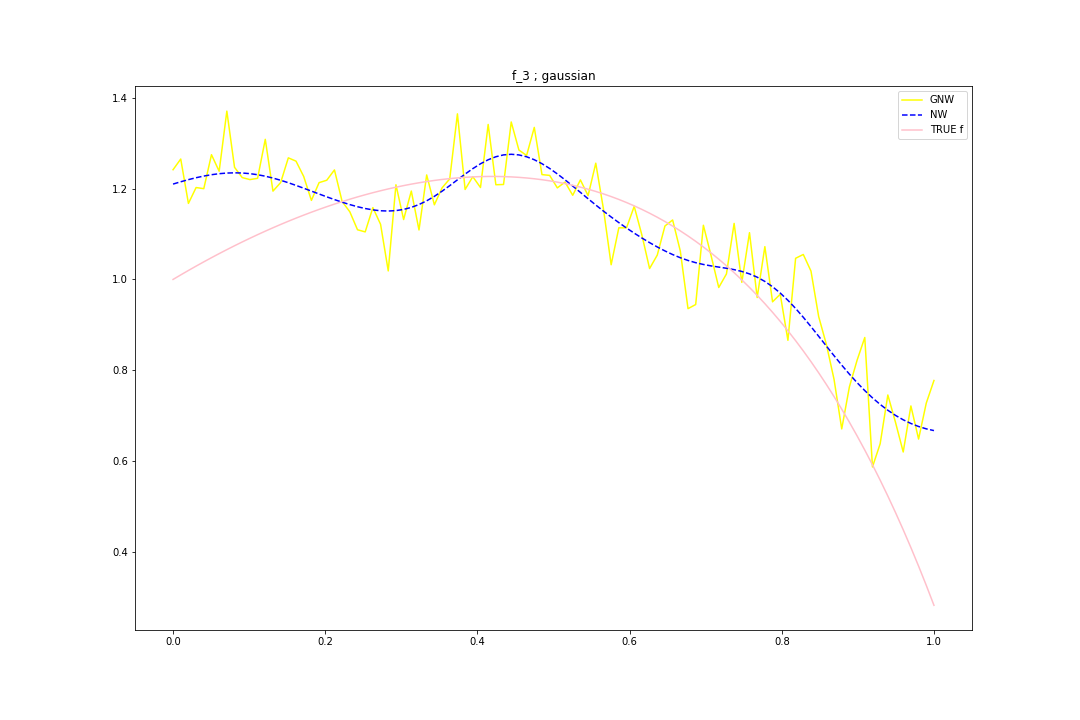
\includegraphics[width=0.4\textwidth]{SSLAN_f_3_gaussian.png}
    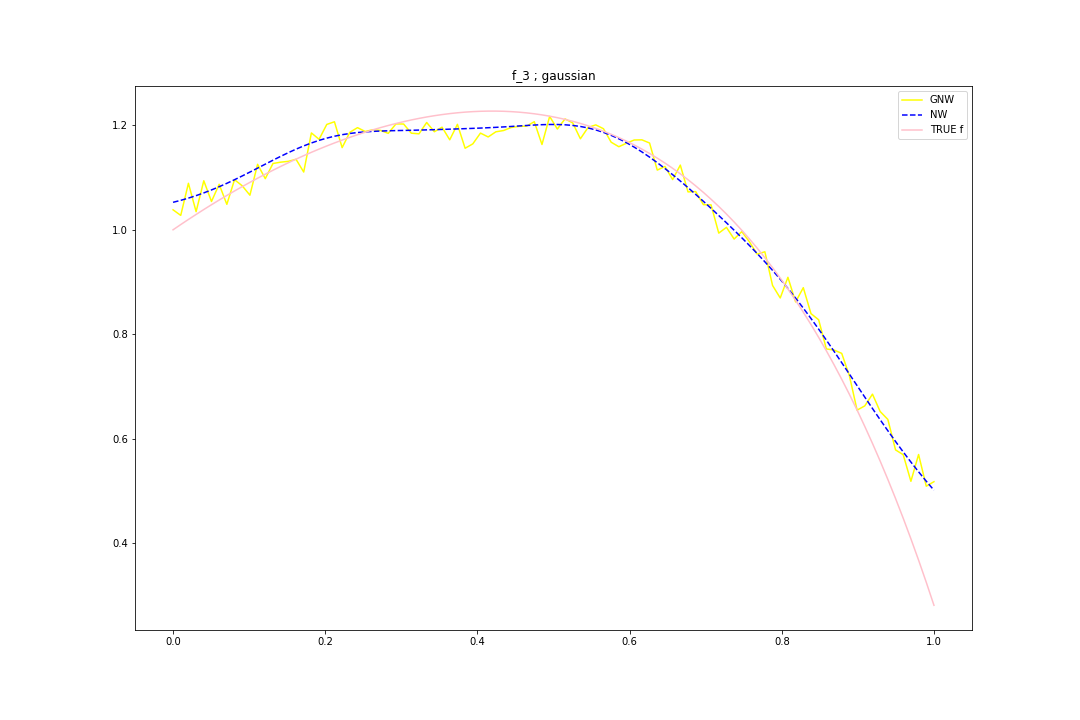
\includegraphics[width=0.4\textwidth]{MSMN_f_3_gaussian.png}
    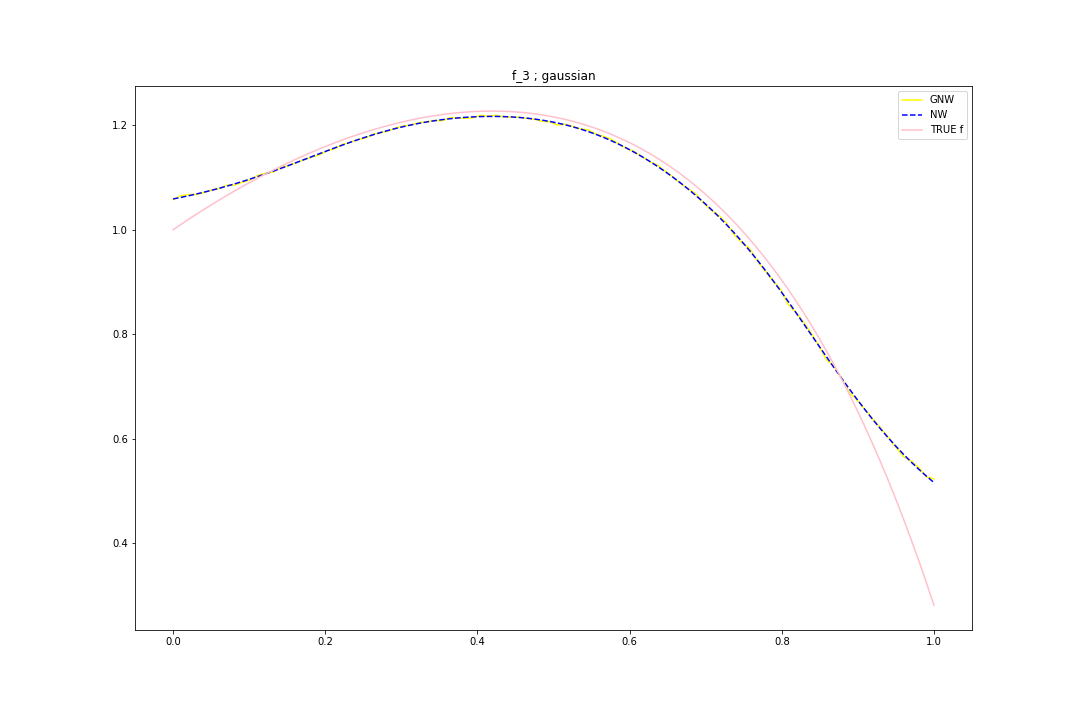
\includegraphics[width=0.4\textwidth]{LSLN_f_3_gaussian.png}
    \caption{Comparison of GNW and NW}
    \label{fig:simulations}
\end{figure}
\end{block}
\end{column}
\end{columns}
\end{frame}
\end{document}